\documentclass[../lab2.tex]{subfiles}

\begin{document}
\subsection{Test TCP - Singolo flusso, full duplex}
\begin{center}
    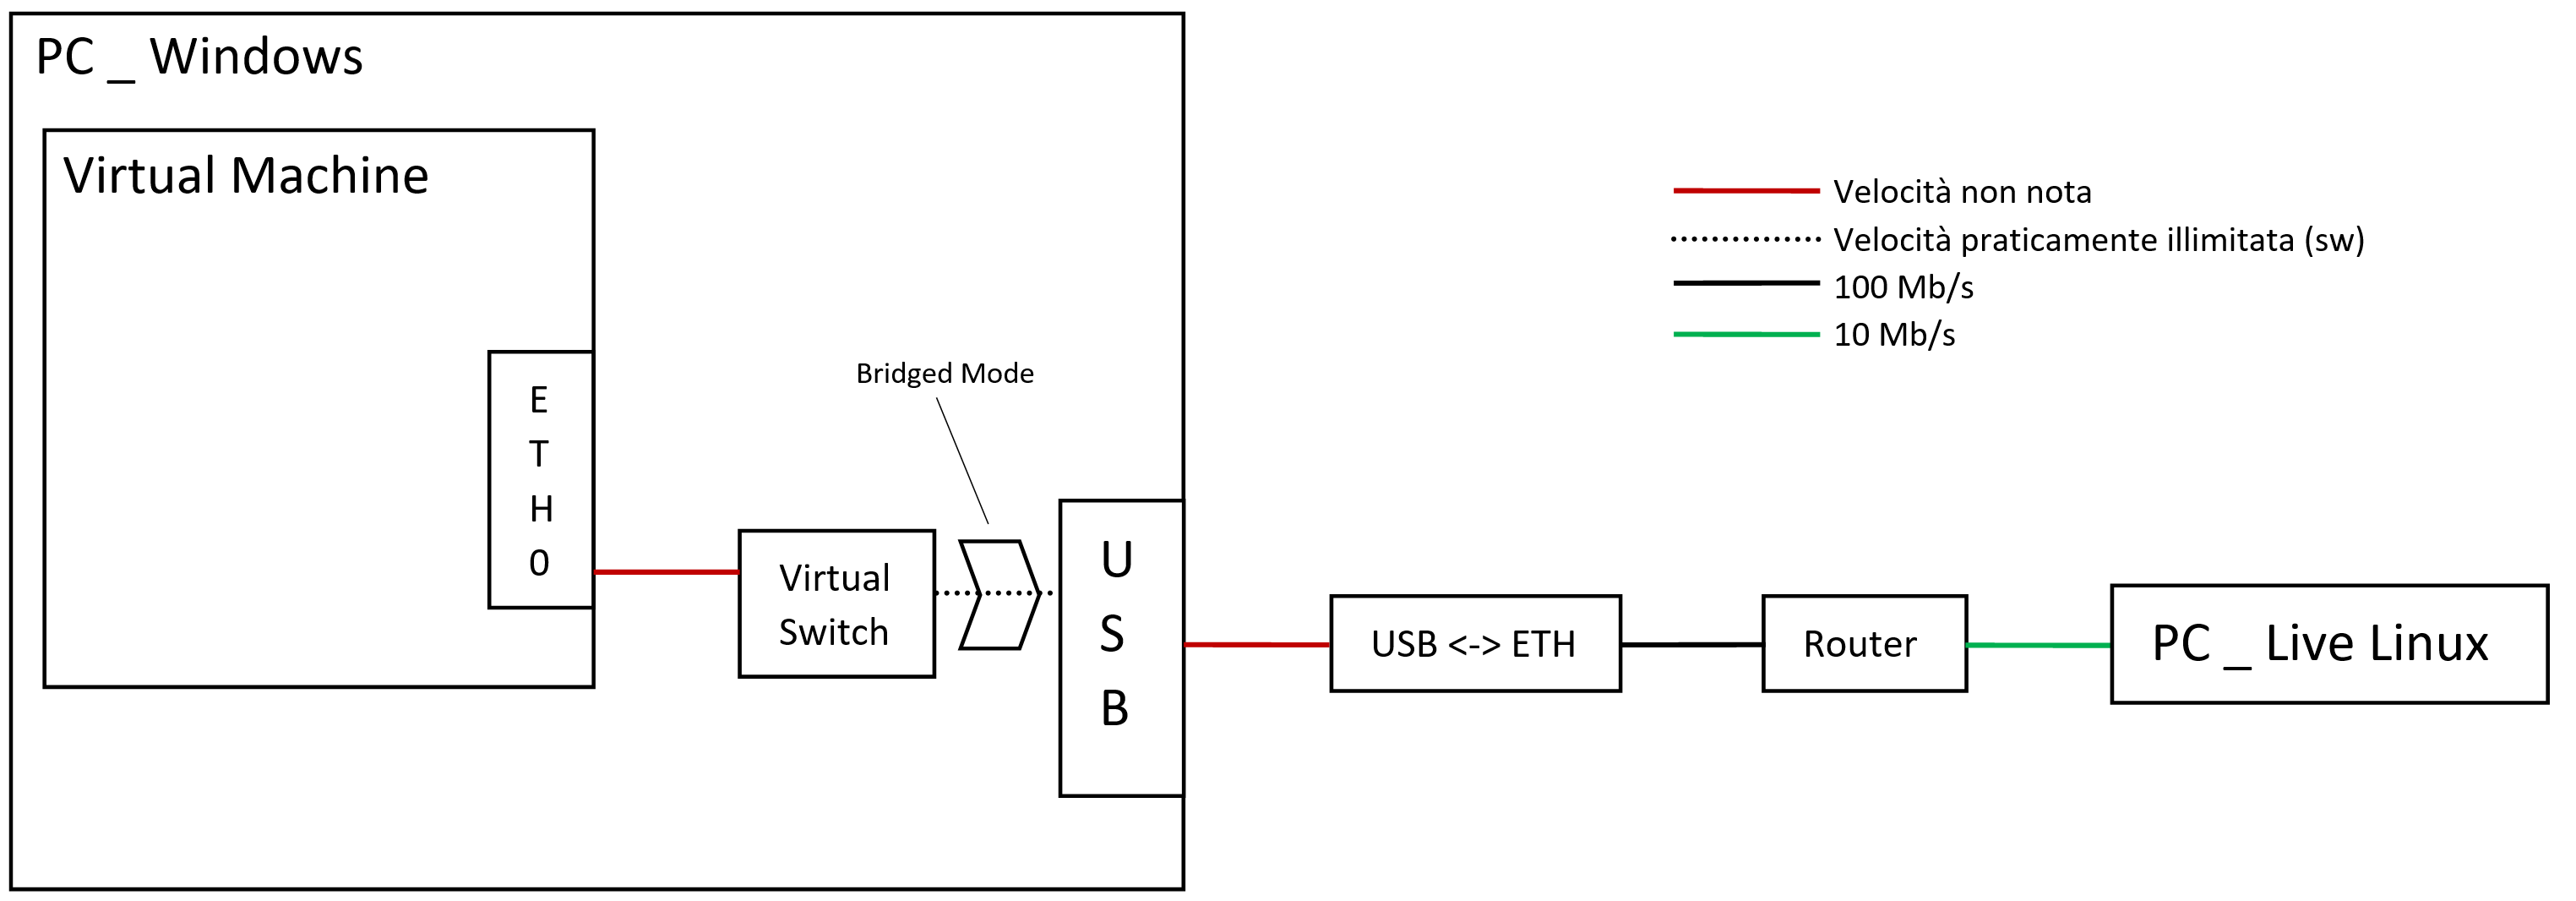
\includegraphics[scale=0.10]{Config1.png}
\end{center}
     
    In questo primo scenario si collegano due pc, uno con live Linux (Ubuntu) e un altro con
    Windows, tramite router. L'assegnazione degli indirizzi è lasciata al DHCP del router,
    si imposta inoltre la velocità dell'interfaccia di rete tra pc Linux e router a 10Mb/s
    per semplicità di analisi: \textit{"sudo ethtool -s eth0 speed 10 duplex full autoneg on"}.
    Per questo primo test si esegue il comando \textit{iperf3 -s} per abilitare il server
    su Windows e \textit{iperf3 -c 192.168.1.196} per aprire una connessione tra pc Linux (client)
    e server. Sono lasciate le opzioni di default dell'applicazione \textit{iperf}:
    \begin{itemize}
        \item la durata del test è di 10 secondi, così da rendere trascurabile lo \textit{store and forward} del router
        \item la lunghezza dei dati generati è pari ad un MSS, ovvero 1460 byte a livello applicazione (L7)
    \end{itemize}
    Utilizzando (2) si può prevedere l'efficienza del canale e di conseguenza la velocità ottenuta con \textit{iperf3}.
    \begin{equation}
        \centering
        V_{MAX} = \frac{MSS}{MSS+20+20+38} \cdot C \simeq 9.5 Mb/s
    \end{equation}
    Prendendo in considerazione anche le opzioni TCP, si ottiene un'efficienza più coerente con i dati otenuti:
    \begin{equation}
        \centering
        V_{MAX} = \frac{MSS}{MSS+32+20+38} \cdot C \simeq 9.41 Mb/s
    \end{equation}
    I problemi a livello fisico sono trascurabili, essendo i due host collegati tramite cavi ethernet di dimensioni ridotte. 
    Non ci aspettiamo collisioni di alcun tipo essendo i canali \textit{full-duplex}. In questo scenario non 
    si dovrebbero generare problemi di congestione poichè il client che comunica con il server ha una velocità di 
    connessione di due ordini di grandezza inferiore, quindi il server sarà in grado di smaltire il traffico
    senza problemi.
\end{document}